\subsection{拓展实验 D：崩溃的根源是“等待被高估”}

\begin{figure*}[t]
	\centering
	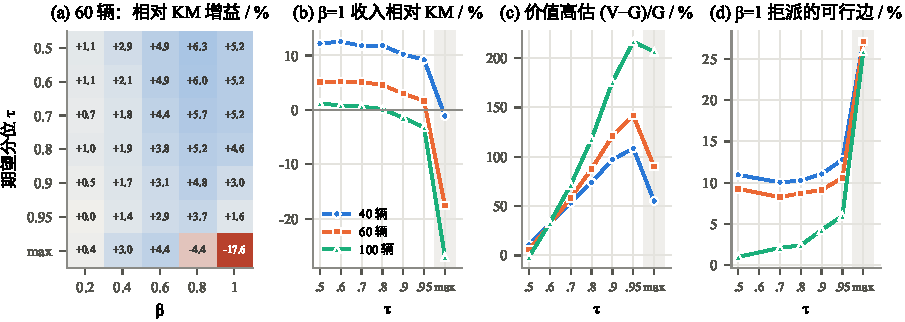
\includegraphics[width=\textwidth]{fig/exp6_expectile.pdf}
	\caption{价值目标乐观度谱（$\Dt=10$ min，3 个训练种子 × 10 个测试日）。(a) 60 辆车时各 $(\tau,\beta)$ 相对 KM 即时收入的增益；(b) $\beta=1$ 时的收入；(c) 价值表相对真实折扣回报的高估（$\beta=0.6$ 策略）；(d) $\beta=1$ 派单时边权 $\le0$、被拒派的可行边比例。灰色区域为 max 目标}
	\label{fig:expectile}
\end{figure*}

\begin{table}[t]
	\centering
	\caption{$\beta=1$ 时可行边上的平均价值项（元，3 种子 × 5 测试日）}
	\label{tab:gostay}
	\small
	\setlength{\tabcolsep}{3pt}
	\begin{tabular}{llcccc}
		\toprule
		车队 & 目标 & 出发 & 等待 & 出发$-$等待 & 出发/等待 \\
		\midrule
		\tabinput{tables/exp6b.tex}
		\bottomrule
	\end{tabular}
\end{table}

拓展 B 把 Q-KM 的崩溃归因于 max 目标的过估计。如果这一解释成立，那么任何足够乐观的目标都应当同样崩溃。\Cref{fig:expectile} 用期望分位目标检验了这个推论，结果与之相反。

\textbf{高估的幅度不能解释崩溃。} 随着 $\tau$ 增大，价值表的高估单调上升（\cref{fig:expectile}(c)）。$\tau=0.95$ 时高估达到 109\%/142\%/217\%（40/60/100 辆），与 max 目标的 55\%/90\%/206\% 相当，甚至更高。但 $\tau=0.95$ 在 $\beta=1$ 时的收入仍为 KM 的 $+9.2$\%/$+1.6$\%/$-3.2$\%，而 max 目标是 $-1.1$\%/$-17.6$\%/$-27.0$\%（\cref{fig:expectile}(b)）。在各自最佳的 $\beta$ 下，$\tau$ 从 0.5 增大到 0.95 只让增益平滑地下降 1.2–2.5 个百分点，热力图上也看不到 max 目标在右下角出现的断崖（\cref{fig:expectile}(a)）。

\textbf{决定性的是高估落在哪里。} \Cref{tab:gostay} 把边权中的长期项拆成“出发”$\gamma^{\Delta}V(t{+}\Delta,k)$ 与“等待”$\gamma V(t{+}1,i)$。期望分位目标把两者近似同比例放大：$\tau$ 从 0.5 到 0.95，出发/等待之比始终在 0.88–0.93 之间，因而在边权的差分中大部分相互抵消。max 目标则不同：与 $\tau=0.95$ 相比，它的出发价值低 5.8–10.9 元，等待价值只低 0.1–7.0 元，出发/等待之比降到 0.84，长期项从 PE 的 $-2.3$ 至 $-6.4$ 元扩大到 $-11.7$ 至 $-12.3$ 元。结果有 26\%–27\% 的可行边被判为负权而不派（\cref{fig:expectile}(d)），而期望分位目标下这一比例不超过 13\%。

\textbf{一个解释：max 的乐观按决策时点累积。} Q-learning 的目标在每个决策时点对 $\mathcal{A}(s')\cup\{\text{等待}\}$ 取一次 max，等于假设司机下一时刻总能接到附近最好的订单。原地等待的司机每 10 分钟就经历一个决策时点，送客的司机在 $\Delta$ 个时间片里只在到达时经历一次。因此单位时间内，等待状态积累的乐观远多于出发状态，平台被系统性地诱导去“等更好的单”。期望分位的乐观则作用在每次更新所采样的回报上，等待转移的回报几乎是确定的（无收入、仍在原区域），不会因决策时点多而额外放大。这一解释与\cref{tab:gostay} 中“max 只压低出发/等待之比”的现象一致，但严格验证还需要控制决策频率的对照实验。这一结论说明，改进长期价值派单的关键不在于压低价值的整体水平，而在于保证不同动作之间的\textbf{相对}价值无偏。
